\documentclass[10pt]{amsart}
\usepackage{geometry}                % See geometry.pdf to learn the layout options. There are lots.
\geometry{letterpaper}                   % ... or a4paper or a5paper or ... 
%\geometry{landscape}                % Activate for for rotated page geometry
%\usepackage[parfill]{parskip}    % Activate to begin paragraphs with an empty line rather than an indent
\usepackage{graphicx}
\usepackage{amssymb}
\usepackage{epstopdf}

%%%%%%%%%%%%%%%pretty code start%%%%%%%%%%%%%%%%%%%%%%%%
\usepackage[scaled]{beramono}
\usepackage{color}
\usepackage{listings}
\usepackage{setspace}

\definecolor{Code}{rgb}{0,0,0}
\definecolor{Decorators}{rgb}{0.5,0.5,0.5}
\definecolor{Numbers}{rgb}{0.5,0,0}
\definecolor{MatchingBrackets}{rgb}{0.25,0.5,0.5}
\definecolor{Keywords}{rgb}{0,0,1}
\definecolor{self}{rgb}{0,0,0}
\definecolor{Strings}{rgb}{0,0.63,0}
\definecolor{Comments}{rgb}{0,0.63,1}
\definecolor{Backquotes}{rgb}{0,0,0}
\definecolor{Classname}{rgb}{0,0,0}
\definecolor{FunctionName}{rgb}{0,0,0}
\definecolor{Operators}{rgb}{0,0,0}
\definecolor{Background}{rgb}{0.98,0.98,0.98}

\lstnewenvironment{python}[1][]{
\lstset{
numbers=left,
numberstyle=\footnotesize,
numbersep=1em,
xleftmargin=1em,
framextopmargin=2em,
framexbottommargin=2em,
showspaces=false,
showtabs=false,
showstringspaces=false,
frame=l,
tabsize=4,
% Basic
basicstyle=\ttfamily\small\setstretch{1},
backgroundcolor=\color{Background},
language=Python,
% Comments
commentstyle=\color{Comments}\slshape,
% Strings
stringstyle=\color{Strings},
morecomment=[s][\color{Strings}]{"""}{"""},
morecomment=[s][\color{Strings}]{'''}{'''},
% keywords
morekeywords={import,from,class,def,for,while,if,is,in,elif,else,not,and,or,print,break,continue,return,True,False,None,access,as,,del,except,exec,finally,global,import,lambda,pass,print,raise,try,assert},
keywordstyle={\color{Keywords}\bfseries},
% additional keywords
morekeywords={[2]@invariant},
keywordstyle={[2]\color{Decorators}\slshape},
emph={self},
emphstyle={\color{self}\slshape},
%
}}{}

\newcommand{\prettycode}[2]{
  \hrulefill
  \subsection*{#1}
  \lstinputlisting{#2}
  \vspace{2em}
}
%%%%%%%%%%%%%%%pretty code end%%%%%%%%%%%%%%%%%%%%%%%%

\DeclareGraphicsRule{.tif}{png}{.png}{`convert #1 `dirname #1`/`basename #1 .tif`.png}

\title{STA 250: HW2: Big Data Module}
\author{Christopher Conley}
\date{}                                           % Activate to display a given date or no date

\begin{document}
\maketitle
\doublespacing
\tableofcontents
\section{Question 1: Bag of Little Bootstraps (BLB) }

\begin{figure}[htbp] %  figure placement: here, top, bottom, or page
   \centering
   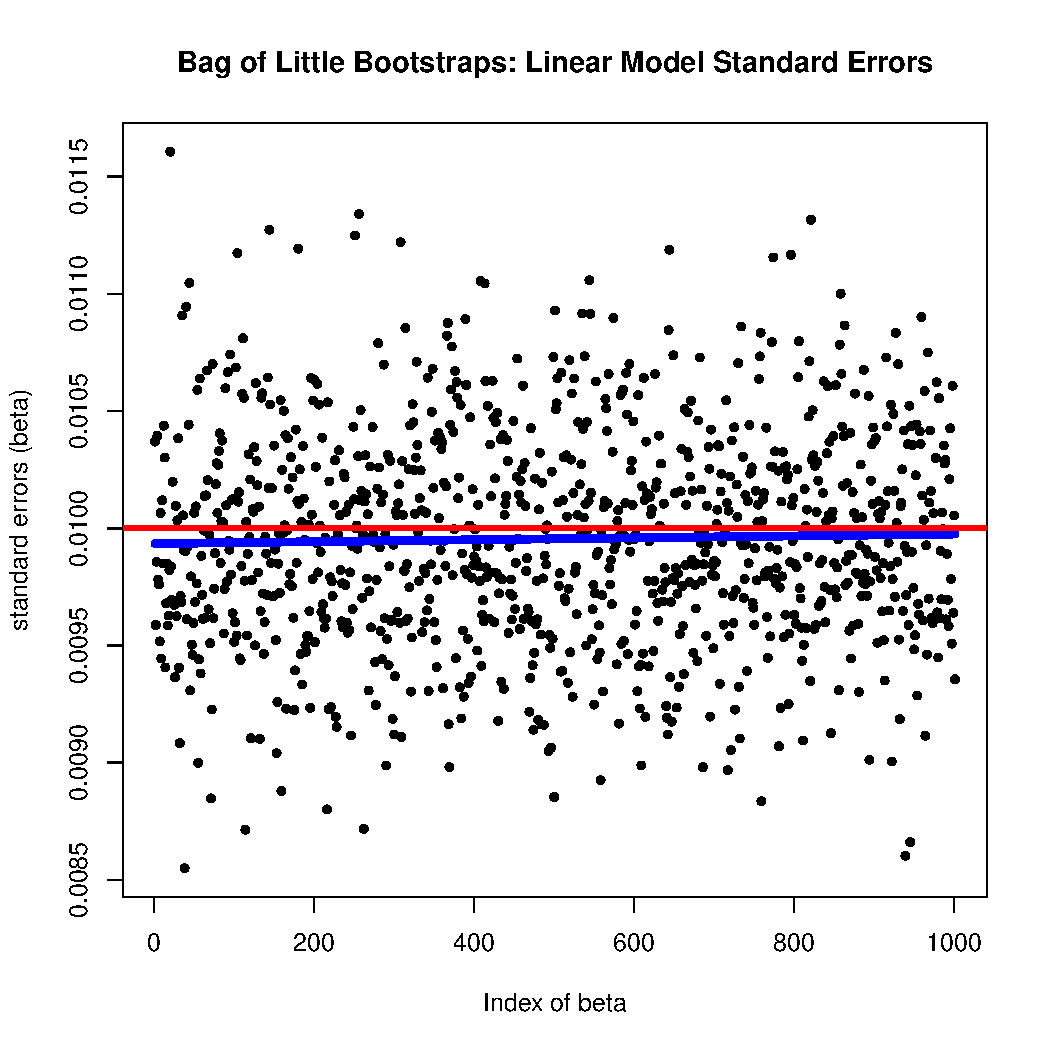
\includegraphics[width=3in]{../BLB/blb_lin_reg_se.pdf} 
   \caption{The standard errors (s.e)  of the linear regression coefficients, $\beta$ produced by BLB.  They are centered near the red line at 0.01, representing the expected neighborhood of the s.e.  The blue line is the cross-validated cubic spline smoothed fit to the BLB s.e. which is very close in proximity to the red line. }
   \label{fig:blb}
\end{figure}

\subsection{Why BLB over other methods}

The BLB algorithm provides robust quality assessment (i.e. standard errors) of an estimator with the same properties as the bootstrap (e.g.  asymptotic consistency) with a focus on being highly scalable to large data sets on distributed computing environments. For big data, the bootstrap was computationally burdensome to repeatedly resample a data set of the original size hundreds of times, where estimation could take days or longer. Work to reduce number of resamples (Efron 1988, Efron \& Tibshirani 1993), or other modifications such as the subsampling (Politis et al. 1997) and m out of n bootstrap (Bickel 1997) have failed to reduce the computational burden and still remain entirely robust. With m out of n bootstrap, knowledge of the convergence rates of the estimator is needed for rescaling purposes because the variability of the subsample is different from the whole data set. Extra mathematical conditions such as these limited the practical implementation of this general tool. Kleiner \emph{et al.} successfully proposed an automatic, accurate, and highly scalable version of the Bootsrap. 

\subsection{What the BLB does}

Let $n$ be the size of the original data set. 

\begin{enumerate}
\item Split the data into $1,\dots,S$ subsamples of size $b < n$.
\item For each subsample of at most $b$ unique data points, resample with replacement to the size of the original data set $1,\dots,R$ times according to a Multinomial with equal probability on the $b$ outcomes. 
\item Compute the quality assessment of the estimator (i.e. standard error) on the R estimates within the subsample.
\item Average over the S standard errors to get the final quality assessment of the estimator. 
\end{enumerate}

\subsection{Key Computational Advantage}

Although the size the subsamples $b << n$ might appear to introduce bias, the weighted resampling based on the Multinomial weights gives the effect of sampling on the scale of the original data set size without the added computational burden or the need for rescaling the quality assessment. In the application of multiple linear regression on  1 million observations with 1K covariates, the subsamples is on the order of thousands (i.e $b = n^{0.7} \approx 1,500$), but the multinomial-weighted least squares fit represents a resample of the larger data set, yet is very computationally efficient because the number of unique observations is at most, the size of b. 

%%%%%%%% Insert code %%%%%%%%%%%%%%%%%%%
Utility Functions
\prettycode{BLB-utils}{../BLB/BLB_utils.R}
Running the BLB.
\prettycode{BLB-linear-regression}{../BLB/BLB_lin_reg_job.R}



\section{Question 2: MapReduce for bivariate histogram}


\begin{figure}[htbp] %  figure placement: here, top, bottom, or page
   \centering
   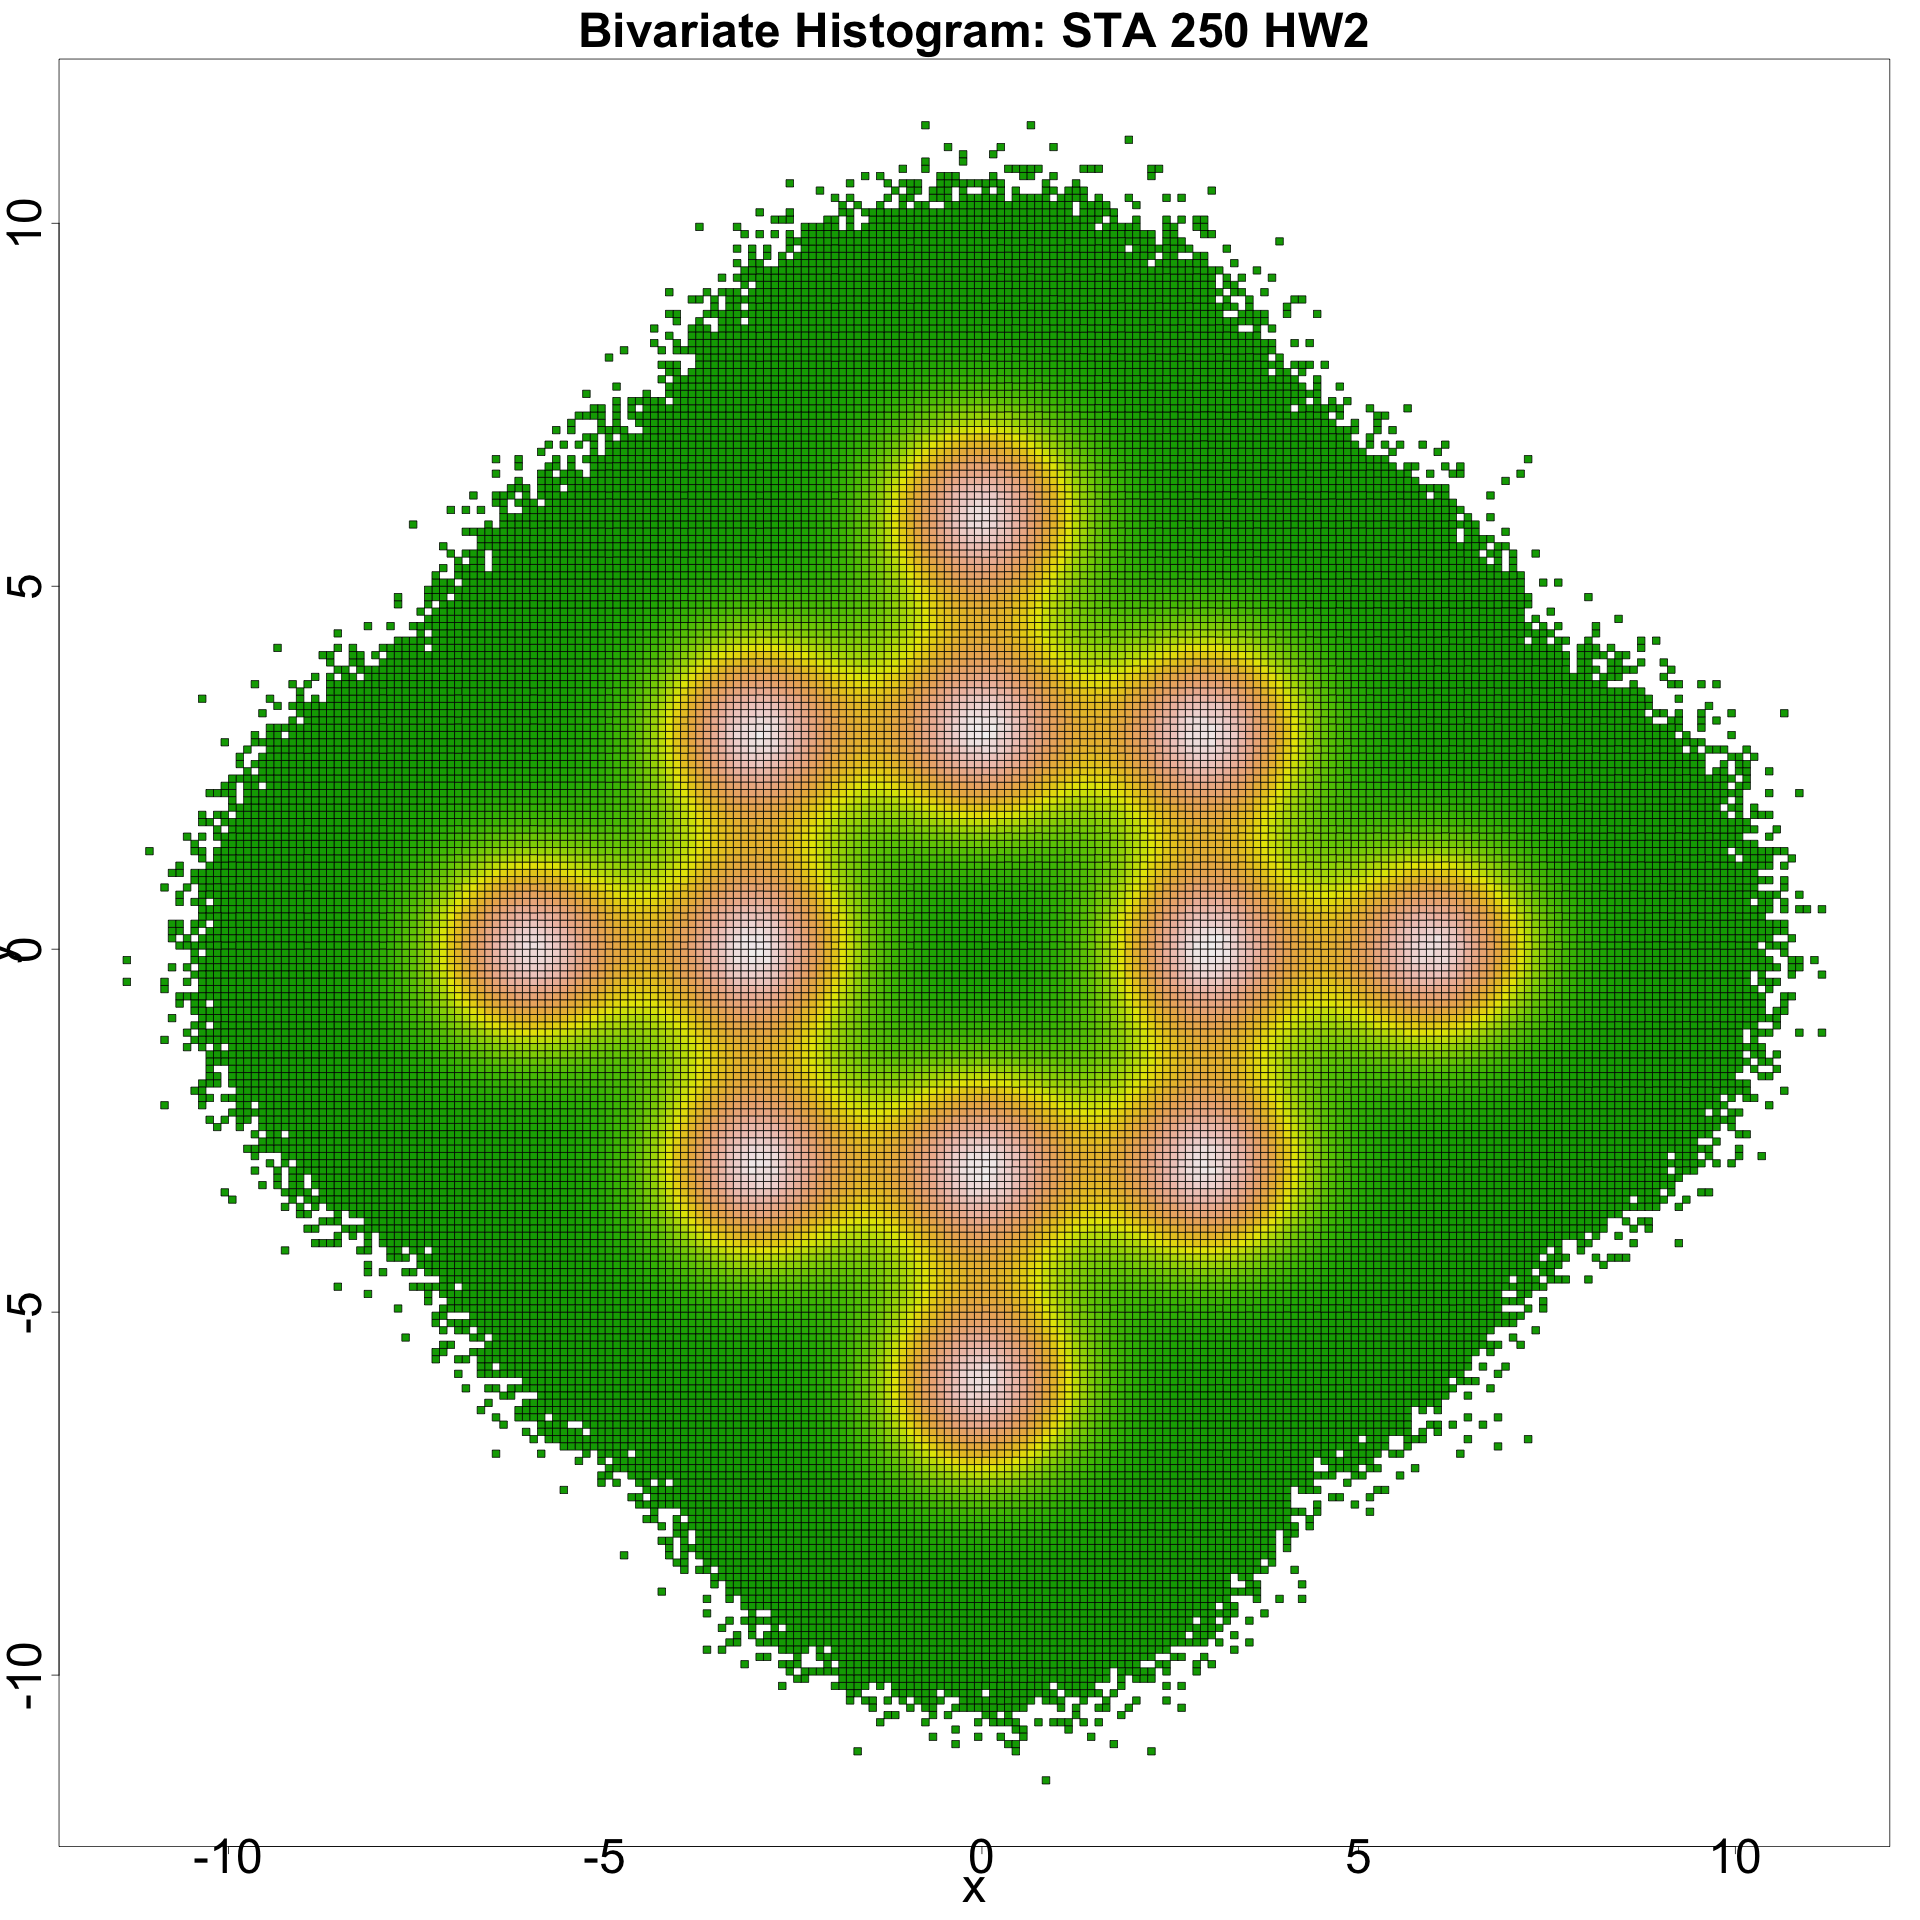
\includegraphics[width=3in]{../Streaming/hist2d.png} 
   \caption{The bivariate histogram of the full data set which was computed on the Hadoop Distributed File System on Amazon Elastic Map Reduce framework. }
   \label{fig:hist2d}
\end{figure}

\subsection{Map}

The mapping task was to associate each $(x,y) \in R^2$ in a 2-dimensional bin. The mapper implemented was highly abstracted and could be applied to a a $D$ dimensional histogram.  Further, I was careful to implement an ``if'' clause to catch the case when a number fell on the boundary (e.g. 5.5 should be in the bin 5.4 to 5.5) and forced what has been termed as ``left inclusion''. The map function separated the low and high bin boundaries with commas to keep the key value as similar to the desired output in the end.

%%%%%%%% Insert mapper.py code %%%%%%%%%%%%%%%%%%%
\prettycode{Mapper}{../Streaming/mapper.py}

\subsection{Reduce}

The problem structure of the reducer was so similar to the example in class; only instead of counting words, the task was to count the frequency of pre-sorted bin occurrences . Only a minor modification was made to the lecture code, where the final count of the bins was delimited with the key by a comma. Everything else was kept as is. While this code could be improved, it sufficed for this exercise. Because of the similarity of the code, it was relegated to the appendix.

\subsection{Performance \& Improvements}

The code took $\approx 20$ minutes to run. As I am not a ``pythonista'', certainly improvements could be made to improve the readability and speed. Its hard to know what those improvements might be since ``ignorance is bliss''. 


\subsection{Amazon Elastic Map Reduce Session Commands}
\prettycode{Reducer}{../Streaming/my_aws_hadoop_hw_session.sh}

\section{Question 3: Hive Basics}

The following code was used generate the within group means and variances. Its primary advantage is that it could read in a tab-delimited file of arbitrarily many columns without explicit declaration. The limitation of the code is that the output of the hive querying code is not formatted appropriately and my efforts to write out to an external table that was formatted correctly did not work. 


\begin{figure}[htbp] %  figure placement: here, top, bottom, or page
   \centering
   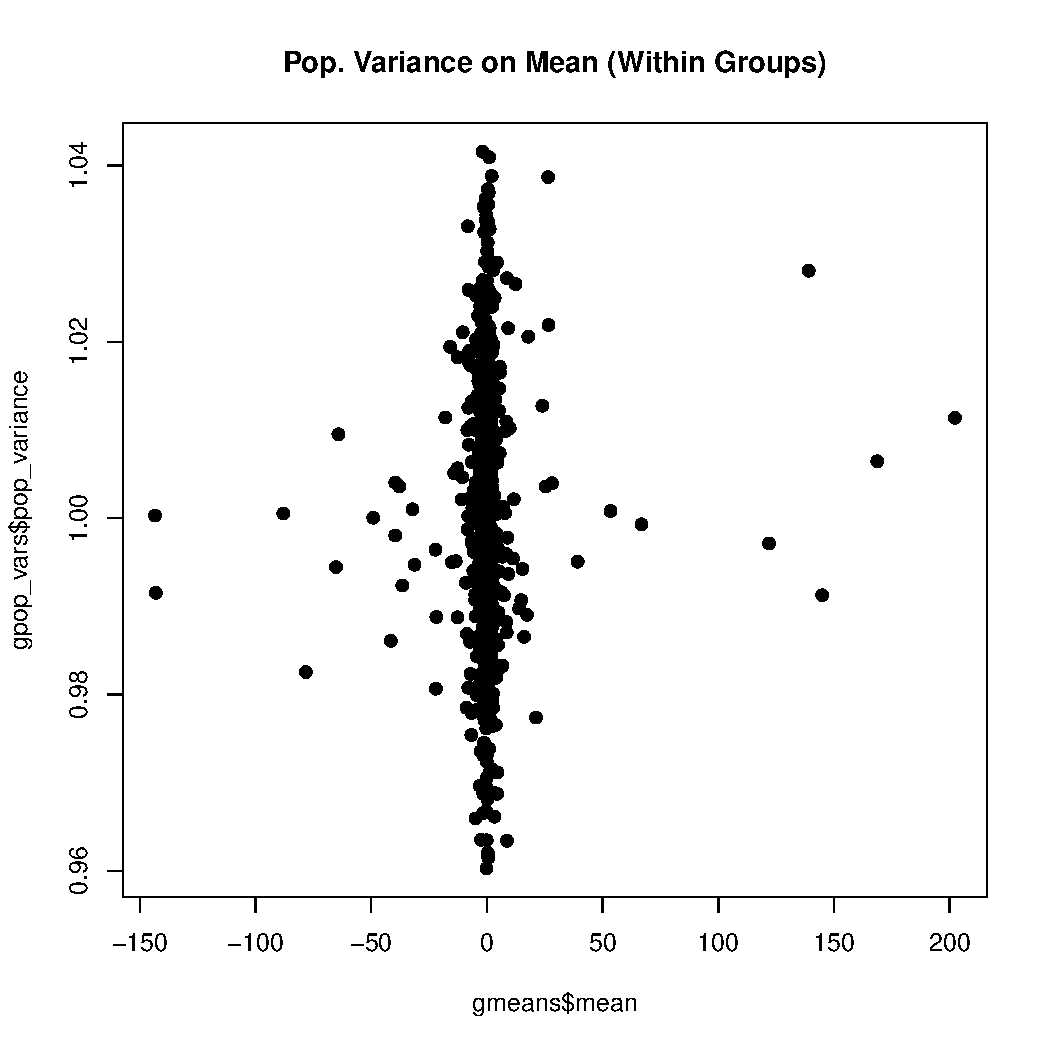
\includegraphics[width=3in]{../HiveBasics/mean_on_var.pdf} 
   \caption{The variance (y-axis) is plotted against  the mean(x-axis). The within-group means are centered at zero and the within-group variance is centered about 1. There appears  to be no obvious dependence between the withing-group mean and variances. This plot contains the population estimates of the variances. }
   \label{fig:hivebasics}
\end{figure}

\newpage

\subsection{Amazon Hive Session Commands}

\prettycode{Hive Basics}{../HiveBasics/within_stats.sh}


\section{Appendix A: Reducer Code}


%%%%%%%% Insert reducer.py code %%%%%%%%%%%%%%%%%%%

\prettycode{Reducer}{../Streaming/reducer.py}


\end{document}  